\documentclass[tikz,border=10pt]{standalone}
\usepackage[charter]{mathdesign}
\begin{document}
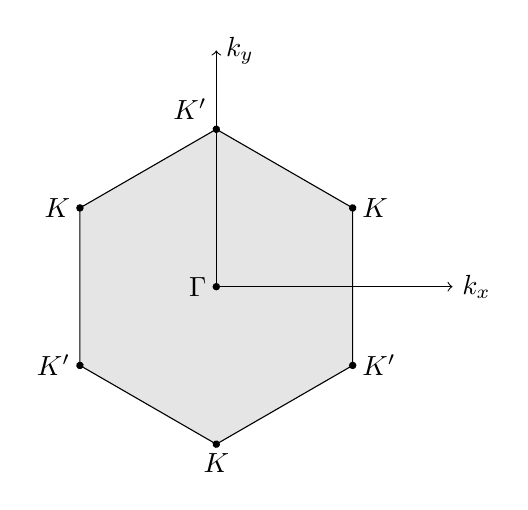
\begin{tikzpicture}[x=2cm,y=2cm]
\def\sq{0.866025}
\coordinate (K) at (1.1*0.5, 1.1*\sq);
\draw[fill=black!10, rotate around={-30:(0,0)}](1,0) -- (0.5, \sq) -- (-0.5, \sq) -- (-1,0) -- (-0.5, -\sq) -- (0.5, -\sq) -- cycle;
\draw[fill=black, rotate around={-30:(0,0)}] (0.5, \sq) circle (0.02) node[right] {$K$};
\draw[fill=black, rotate around={-150:(0,0)}] (0.5, \sq) circle (0.02) node[below] {$K$};
\draw[fill=black, rotate around={90:(0,0)}] (0.5, \sq) circle (0.02) node[left] {$K$};
\draw[fill=black, rotate around={30:(0,0)}] (0.5, \sq) circle (0.02) node[above left] {$K'$};
\draw[fill=black, rotate around={-90:(0,0)}] (0.5, \sq) circle (0.02) node[right] {$K'$};
\draw[fill=black, rotate around={150:(0,0)}] (0.5, \sq) circle (0.02) node[left] {$K'$};
\draw[fill=black] (0,0) circle (0.02) node[left] {$\Gamma$};
\draw[->] (0,0) -- (1.5,0) node [right] {$k_x$};
\draw[->] (0,0) -- (0,1.5) node [right] {$k_y$};
\end{tikzpicture}
\end{document}